\chapter{Implementing Internal Model Controller for first order systems on a Single Board Heater System}
The Aim of this experiment is to implement an Internal Model Controller for first order systems on a single board heater system. The target group is anyone who has basic knowledge of Control Engineering.
\begin{figure}
	\centering
		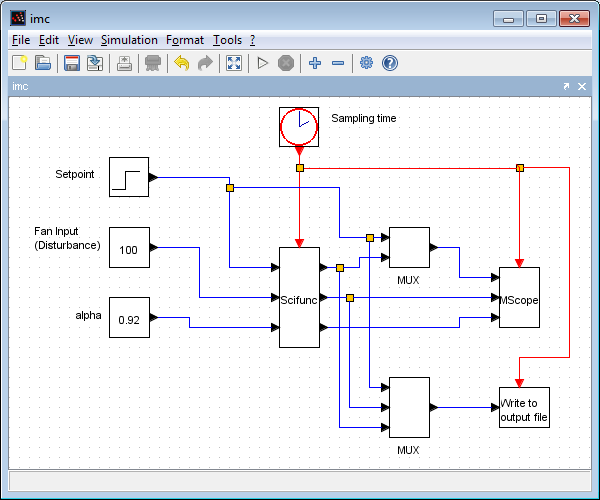
\includegraphics[width=\linewidth]{IMC/imc_xcos.png}
	\caption{Xcos interface for this experiment}
	\label{Xcos_imc}
\end{figure}
We have used Scilab with Xcos as an interface for sending and receiving data. This interface is shown in Fig.\ref{Xcos_imc}.Fan speed and Heater current are the two inputs to the system. For this experiment, the heater current is used as a control effort. The fan input could be thought of as an external disturbance.

\section{IMC Design for Single Board Heater System}
Internal Model Controller contain explicit model of plant as its part, hence it is name as Internal Model Controller \cite{kmm09}. 
With stable open loop transfer function and stable controller, the closed loop system can be stabled. The IMC has been used mainly for stable plants.
\begin{figure}
\begin{center}
\begin{tikzpicture}[auto,node distance=2cm]
\node[input](input){};
\node[sum,right of=input](sum1){};
\draw[->](input)--node{$r$}(sum1);
\node[block,right of=sum1](gqz){$G_Q(z)$};
\draw[->](sum1)--node{$e$}(gqz);
\node[branch,right of=gqz, node distance=2cm](b1){};
\node[block, right of=b1](gpz){$G_p(z)$};
\draw[->](gqz)--node{$u$}(gpz);
\node[sum, right of=gpz,pin={[pinstyle] above:$\xi$},node distance=2cm](sum2){};
\draw[->](gpz)--(sum2);
\node[output, right of=sum2](output){};
\draw[->](sum2)--node{$y$}(output);
\node[branch, right of=sum2, node distance=1cm](b2){};
\node[sum, below of=b2,node distance=2cm](sum3){};
\draw[->](b2)--(sum3);
\node[block,below of=gpz](gz){$G(z)$};
\draw[->](b1)|-(gz);
\draw[->](gz)--node{$\bar{y}$\hspace{0.7cm} $-$}(sum3);
\draw[->](sum3)--(10,-3)-|node[pos=0.88]{$-$}(sum1);
\end{tikzpicture}
\end{center}
\caption{IMC feedback configuration}
\label{imcfeedback}
\end{figure}

Now, transfer function of the stable plant be denoted by $G_p (z)$ and it's model is denoted by $G(z)$,hence
\begin{align}
y(n)=G(z)u(n)+\xi(n) 
\end{align}
where; \\
y(n)=plant output;\\
      u(n)=plant input;\\
      $\xi$(n)=noise.
      
Fig.\ref{imcfeedback} shows method to control stable plant by using internal model control.
For noise rejection with y=0 we required $G_Q=G_p^{-1}$ and $G=G_p$ i.e. for stable $G_Q$ we required an approximate inverse of G.Also, for internal stability transfer function between any to points in the feedback loop must be stable.\cite{kmmdc09}
\begin{figure}
\begin{center}
\begin{tikzpicture}[auto,node distance=2cm]
\node[input](input){};
\node[sum,right of=input](sum1){};
\draw[->](input)--node{$r$}(sum1);
\node[sum, right of=sum1](sum2){};
\draw[->](sum1)--(sum2);
\node[block,right of=sum2](gqz){$G_Q(z)$};
\draw[->](sum2)--node{$e$}(gqz);
\node[branch,right of=gqz, node distance=2cm](b1){};
\node[block, right of=b1](gpz){$G_p(z)$};
\draw[->](gqz)--node{$u$}(gpz);
\node[sum, right of=gpz,pin={[pinstyle] above:$\xi$},node distance=2cm](sum3){};
\draw[->](gpz)--(sum3);
\node[output, right of=sum3](output){};
\draw[->](sum3)--node{$y$}(output);
\node[block, below of=gqz](gz){$G(z)$};
\draw[->](b1)|-(gz);
\draw[->](gz)-|(sum2);
\draw[->](sum3)--(10,-3)-|node[pos=0.88]{$\bar{\xi}$}(sum1);
\end{tikzpicture}
\end{center}
\caption{IMC feedback configuration}
\label{feedback}
\end{figure}

\section{Step for designing IMC for stable plant}
Invert the delay free plant model so that $G_Q$ is realizable. For non-minimum phase part of the plant, reciprocal polynomial is use for stable controller. Negative real part of the plant should replace with the steady state equivalent of that part to avoid oscillatory nature of control effort. Low pass filter must use to avoid the high frequency components because of model mismatch.
IMC design means obtaining a realizable $G_Q$ that is stable and approximately inverse of G.
Invert the delay free plant model so that $G_Q$ is realizable. We have model of SBHS ,which is given by,
\begin{align}
	G&=Z^{-1} \frac{0.01163}{1-0.9723Z^{-1}}
\intertext{Inverting delay free plant, We get}
\frac{A}{B}&=\frac{1-0.9723Z^{-1}}{0.01163}
\intertext{Now, Comparing plant model with equation,}
G&=Z^{{-1}}\frac{B^g B^- B^{nm+}}{A}\\
B^g&=0.01163\\
B^-&=1\\
B^{nm+}&=1\\
A&=1-0.9723Z^{-1}
\intertext{For the stable system internal model controller is give by}
G_Q&=\frac{A}{B^gB^-_s B_r^{nm+}}G_f\\
G_Q&=\frac{1-0.9723Z^{-1}}{0.01163}\frac{1-\alpha}{1-\alpha Z^{-1}}
\intertext{Now,}
G_c&=\frac{G_Q}{1-GG_Q}\\
\frac{u}{e}&=\frac{\frac{1-0.9723Z^{-1}}{0.01163}\frac{1-\alpha}{1-\alpha Z^{-1}}}{1-Z^{-1}\frac{0.01163}{1-0.9723Z^{-1}}\frac{1-0.9723Z^{-1}}{0.01163}\frac{1-\alpha}{1-\alpha Z^{-1}}}\\
\intertext{After simplifying, We get}
\frac{u}{e}&=\frac{1-\alpha}{0.01163}\frac{1-0.9723Z^{-1}}{1-Z^{-1}}\\
\frac{u}{e}&=b\frac{1-0.9723Z^{-1}}{1-Z^{-1}}
\intertext{Where,}\\
b&=\frac{1-\alpha}{0.01163}
\intertext{Hence,}
u(n)&=u(n-1)+b[e(n)-0.9723e(n-1)]
\end{align}
For implementing above IMC controller, scilab code is given in {\tt imc.sci} file,listed at the end of this document. Change the current working directory to the folder {\tt imc\_controller}. Execute the file {\tt ser\_init.sce} with the appropriate com port number and then execute the file {\tt imc.sci} for loading the function. Run the xcos file {\tt imc.xcos}. Output of Xcos is shown in below fig.\ref{fig:0.991}. Figure shows three plots. First subplot shows Setpoint and output temperature profile. Second sub plot shows control effort and third subplot shows error between setpoint and plant output.


\section{Experimental Results}
\begin{figure}
	\centering
		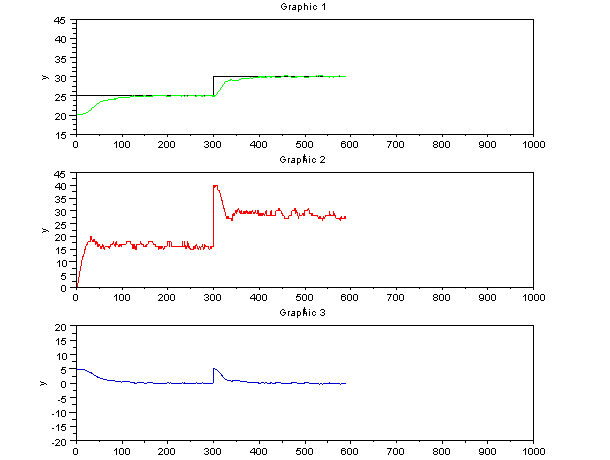
\includegraphics[width=\linewidth]{IMC/imc_092_resp.png}
	\caption{Experimental Results with IMC for $\alpha=0.92$}
	\label{fig:0.991}
\end{figure}
\begin{figure}
	\centering
		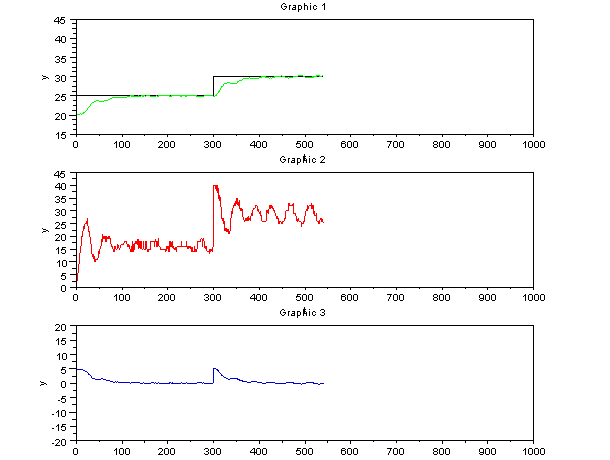
\includegraphics[width=\linewidth]{IMC/imc_085_resp.png}
		\caption{Experimental Results with IMC for $\alpha=0.85$}
	\label{fig:0.98}
\end{figure}
By comparing above two graph we can say that for $\alpha=0.92$ the response of the controller is sluggish. For $\alpha=0.85$ the controller starts responding quickly and no overshoots are seen in the temperature profile.


\subsection{Implementing IMC controller on SBHS, virtually}
The step by step procedure for conducting an experiment virtually is explained in section \ref{vlabsexpt}. The required .sce file is {\tt imc\_virtual.sce}.  You will find this file in the {\tt imc\_controller} directory under {\tt virtual} folder. The necessary codes are listed in the section \ref{imccodes}


\section{Scilab Code}\label{imccodes}
\begin{code}
\ccaption{ser\_init.sce}{\ttfamily ser\_init.sce}
\lstinputlisting{Scilab/local/imc_controller/ser_init.sce}
\end{code}

\begin{code}
 \ccaption{imc.sci}{\ttfamily imc.sci}
\lstinputlisting{Scilab/local/imc_controller/imc.sci}
\end{code}


\begin{code}
 \ccaption{imc\_virtual.sce}{\ttfamily imc\_virtual.sce}
\lstinputlisting{Scilab/virtual/imc_controller/imc_virtual.sce}
\end{code}


\begin{code}
 \ccaption{imc\_virtual.sci}{\ttfamily imc\_virtual.sci}
\lstinputlisting{Scilab/virtual/imc_controller/imc_virtual.sci}
\end{code}


%\bibliography{imc} 
